% Options for packages loaded elsewhere
\PassOptionsToPackage{unicode}{hyperref}
\PassOptionsToPackage{hyphens}{url}
%
\documentclass[
]{article}
\usepackage{amsmath,amssymb}
\usepackage{iftex}
\ifPDFTeX
  \usepackage[T1]{fontenc}
  \usepackage[utf8]{inputenc}
  \usepackage{textcomp} % provide euro and other symbols
\else % if luatex or xetex
  \usepackage{unicode-math} % this also loads fontspec
  \defaultfontfeatures{Scale=MatchLowercase}
  \defaultfontfeatures[\rmfamily]{Ligatures=TeX,Scale=1}
\fi
\usepackage{lmodern}
\ifPDFTeX\else
  % xetex/luatex font selection
\fi
% Use upquote if available, for straight quotes in verbatim environments
\IfFileExists{upquote.sty}{\usepackage{upquote}}{}
\IfFileExists{microtype.sty}{% use microtype if available
  \usepackage[]{microtype}
  \UseMicrotypeSet[protrusion]{basicmath} % disable protrusion for tt fonts
}{}
\makeatletter
\@ifundefined{KOMAClassName}{% if non-KOMA class
  \IfFileExists{parskip.sty}{%
    \usepackage{parskip}
  }{% else
    \setlength{\parindent}{0pt}
    \setlength{\parskip}{6pt plus 2pt minus 1pt}}
}{% if KOMA class
  \KOMAoptions{parskip=half}}
\makeatother
\usepackage{xcolor}
\usepackage[margin=1in]{geometry}
\usepackage{longtable,booktabs,array}
\usepackage{calc} % for calculating minipage widths
% Correct order of tables after \paragraph or \subparagraph
\usepackage{etoolbox}
\makeatletter
\patchcmd\longtable{\par}{\if@noskipsec\mbox{}\fi\par}{}{}
\makeatother
% Allow footnotes in longtable head/foot
\IfFileExists{footnotehyper.sty}{\usepackage{footnotehyper}}{\usepackage{footnote}}
\makesavenoteenv{longtable}
\usepackage{graphicx}
\makeatletter
\def\maxwidth{\ifdim\Gin@nat@width>\linewidth\linewidth\else\Gin@nat@width\fi}
\def\maxheight{\ifdim\Gin@nat@height>\textheight\textheight\else\Gin@nat@height\fi}
\makeatother
% Scale images if necessary, so that they will not overflow the page
% margins by default, and it is still possible to overwrite the defaults
% using explicit options in \includegraphics[width, height, ...]{}
\setkeys{Gin}{width=\maxwidth,height=\maxheight,keepaspectratio}
% Set default figure placement to htbp
\makeatletter
\def\fps@figure{htbp}
\makeatother
\setlength{\emergencystretch}{3em} % prevent overfull lines
\providecommand{\tightlist}{%
  \setlength{\itemsep}{0pt}\setlength{\parskip}{0pt}}
\setcounter{secnumdepth}{-\maxdimen} % remove section numbering
\usepackage{titling}
\pretitle{\begin{center}\Huge\bfseries}
\posttitle{\par\end{center}}
\predate{\begin{center}\large}
\postdate{\par\end{center}}
\preauthor{\begin{center}\large}
\postauthor{\par\end{center}}
\usepackage{amsmath}
\usepackage{amsthm}
\usepackage{rotating}
\ifLuaTeX
  \usepackage{selnolig}  % disable illegal ligatures
\fi
\usepackage{bookmark}
\IfFileExists{xurl.sty}{\usepackage{xurl}}{} % add URL line breaks if available
\urlstyle{same}
\hypersetup{
  pdftitle={Transit Usage in Seattle: A Spatial Investigation},
  pdfauthor={Peter Silverstein},
  hidelinks,
  pdfcreator={LaTeX via pandoc}}

\title{Transit Usage in Seattle: A Spatial Investigation}
\author{Peter Silverstein}
\date{2025-02-22}

\begin{document}
\maketitle

\begin{center}
    {\large Final Project}\\[0.5cm]
    {\large GIS and Spatial Analysis}\\[0.5cm]
    {\large QMSS5070}\\[0.5cm]
    {\large Note that this is a truncated version prepared for an application to the Regional Plan Association}\\[0.5cm]
\end{center}

\newpage

\tableofcontents

\newpage

\section{Introduction}\label{introduction}

\subsection{Research Question:}\label{research-question}

\begin{enumerate}
\def\labelenumi{\arabic{enumi}.}
\tightlist
\item
  How does transit usage percentage (percent of trips using mass transit
  / total trips per census tract) vary spatially in and around Seattle
  and Tacoma, Washington?
\item
  How does this variation relate to population density, median income,
  and median age at the census tract level?
\end{enumerate}

\subsection{Purpose of Study:}\label{purpose-of-study}

There are two purposes to this study. The first is to better understand
where there are concentrations of high and low transit usage around the
region. If there is clustering and we see hotspots and/or coldspots,
further policy-focused questions can be asked.

The second research question is whether three independent variables
(population density, median income, and median age) are related to the
outcome of interest (percentage of commuter trips taken using public
transit).

\subsection{Hypotheses}\label{hypotheses}

\begin{enumerate}
\def\labelenumi{\arabic{enumi}.}
\tightlist
\item
  I believe we will see transit hotspots close to urban centers (e.g.,
  Seattle and Tacoma, the two biggest cities in the region of interest).
  Further, I believe the opposite will be true for coldspots--they
  should exist further outside urban centers.
\item
  I expect that transit use percentage is positively associated with
  population density and median income and negatively associated with
  age.
\end{enumerate}

\section{Data and Methodology:}\label{data-and-methodology}

\subsection{Data Sources:}\label{data-sources}

\begin{enumerate}
\def\labelenumi{\arabic{enumi}.}
\tightlist
\item
  The \textbf{Puget Sound Regional Association (PSRC) Household Travel
  Survey (HTS) 2017-23} is a biennial survey of commuters done in the
  King, Kitsap, Pierce, and Snohomish counties of Washington state (the
  counties surrounding Seattle and Tacoma).
\item
  All \textbf{census tract-level ACS 2022 5-year estimates for
  demographic data and the associated geometries} were accessed via the
  R \texttt{tidycensus} package, which leverages an API connection to
  the US Census Bureau to provide US Census data for a specified
  geographic area.
\item
  Finally, \textbf{Stanford's Cities and Towns of the United States,
  2014} dataset provided point data to allow me to add city labels to my
  maps for reference.
\end{enumerate}

\subsection{Data Preparation/Spatial Data
Management:}\label{data-preparationspatial-data-management}

\subsubsection{Data Cleaning}\label{data-cleaning}

\begin{enumerate}
\def\labelenumi{\arabic{enumi}.}
\tightlist
\item
  \emph{Mass Transit:} included in this category trips that used a metro
  bus, private bus or shuttle, urban rail/light rail, school bus, ferry,
  paratransit, and commuter rail. Essentially I included any
  multi-occupancy transit vehicle.
\item
  \emph{Personal Vehicle:} trips including all single-occupancy motor
  vehicles. This includes personal cars, ride-shares, taxis,
  motorcycles, and car-share services.
\item
  \emph{Active Transit:} included walking, running, biking, and
  skateboarding.
\item
  \emph{Other:} included helicopter/plane, ``other'' responses.
\end{enumerate}

\subsection{GIS Methodology Overview}\label{gis-methodology-overview}

\subsubsection{Manipulation/Analytical Methods
Used}\label{manipulationanalytical-methods-used}

I counted the number of trips inside each census tract, then converted
the total trip and mass transit trip counts to percentage. Finally, I
used a simple join function to associate the counts with their
respective geometries.

For the analysis in this project, I will perform a global cluster
analysis (using Moran's I) and visualize any hot and cold spots using
Getis-Ord Gi*. I will then run a Spatial Lag Model (SLM) regressing mass
transit percentage on population density, median income, and median age.

\subsubsection{Software Used}\label{software-used}

All data loading, cleaning, and manipulation, mapping (both choropleth
and Getis-Ord Gi*), table-creation, regression modeling, and write-up
were performed with R and RStudio.

\newpage

\section{Results and Analysis}\label{results-and-analysis}

\subsection{Exploratory Data Analysis via Choropleth Mapping and
Descriptive
Tables}\label{exploratory-data-analysis-via-choropleth-mapping-and-descriptive-tables}

I will begin the analysis portion of this project with some simple
choropleth maps in order to visualize some of the patterns I'm looking
for will be apparent with a simple eye test.

\begin{figure}
\centering
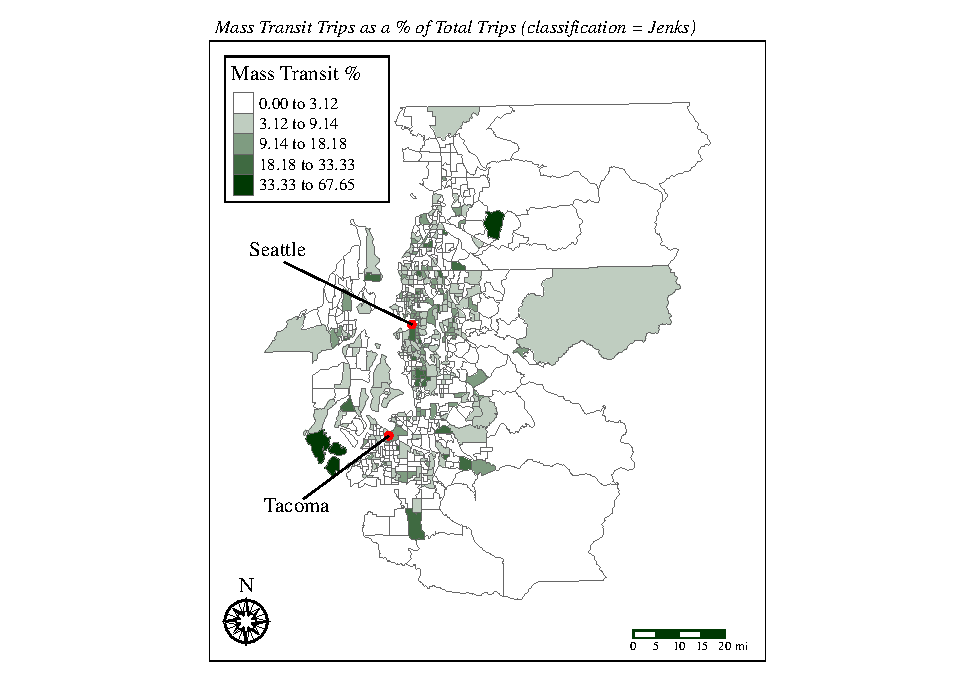
\includegraphics{truncated_transit_hotspots_paper_files/figure-latex/unnamed-chunk-3-1.pdf}
\caption{Sources: US Census ACS 2022 5-year estimates, Puget Sound
Regional Countil, Cities and Towns of the US 2014, via Stanford
University; Classification = jenks}
\end{figure}

Ignoring for a minute the top-end of the scale, it does seem that there
are some clusters with higher transit usage and that these clusters tend
to exist closer to the cities. Not only can we see that the apparent
clustering occurs nearer to the two cities marked on the map, it also
seems as though smaller census tracts tend to have higher mass transit
percentages. As a general rule of thumb, smaller census tracts tend to
be more urban, so this fits with my hypothesis that transit clustering
will occur in more population dense areas.

For the final piece of exploratory data analysis, below is a table
containing basic descriptive statistics for each of my variables. The
only thing I will call out about this table is that it does show the
high number of tracts with 0\% mass transit trips. This is likely due to
a low number of observations in those census tracts, since I only
filtered out tracts with 0 observations. It is entirely possible there
are tracts with a single observation and that the observation is for
personal vehicles, active transit, or other.

\begin{longtable}[]{@{}lrrrr@{}}
\caption{Descriptive Statistics Summary}\tabularnewline
\toprule\noalign{}
& Mass Transit \% & Population Density & Median Income & Median Age \\
\midrule\noalign{}
\endfirsthead
\toprule\noalign{}
& Mass Transit \% & Population Density & Median Income & Median Age \\
\midrule\noalign{}
\endhead
\bottomrule\noalign{}
\endlastfoot
mean & 5.06 & 4,605.37 & 113,140.27 & 39.19 \\
sd & 6.94 & 4,483.13 & 40,662.76 & 5.69 \\
min & 0.00 & 4.90 & 30,327.00 & 21.90 \\
q25 & 0.00 & 1,779.03 & 84,682.75 & 35.60 \\
median & 2.78 & 3,907.93 & 107,472.00 & 38.70 \\
q75 & 7.69 & 5,963.44 & 135,001.75 & 42.60 \\
max & 67.65 & 47,121.04 & 250,001.00 & 69.30 \\
\end{longtable}

\subsection{Cluster Analysis}\label{cluster-analysis}

In this section, I will apply two different methods to test and
visualize the clustering of transit access in the region. First, I will
run a Global Moran's I to determine if the clustering we can see
visually is statistically significant. Then, I will run a hotspot
analysis using the Getis-Ord Gi* statistic, primarily as a tool for
creating a visualization of the clustering.

\subsubsection{Moran's I Test of Global
Clustering}\label{morans-i-test-of-global-clustering}

\begin{verbatim}
## 
##  Moran I test under randomisation
## 
## data:  psrc_table_clean$masstransit_perc  
## weights: weights_clean    
## 
## Moran I statistic standard deviate = 7.1199, p-value = 5.4e-13
## alternative hypothesis: greater
## sample estimates:
## Moran I statistic       Expectation          Variance 
##      0.1928134937     -0.0016103060      0.0007456762
\end{verbatim}

The Global Moran's I value of 0.193 indicates a moderate, positive
clustering pattern. That is, tracts are somewhat likely to be similar to
their immediate neighbors in terms of their mass transit percentage.
High tracts are likely to be bordered by other high tracts, and low
tracts are likely to be bordered by other low tracts. Given that the
Moran's I statistic ranges from -1 to 1, the 0.193 value only indicates
weak-to-moderate positive clustering.

While it is useful to know that there is statistically significant
spatial clustering in our variable of interest with the region, these
statistics alone do a poor job of helping us to understand where this
clustering is happening and whether it fits with expectations. To that
end, I will employ the Getis-Ord Gi* statistic and map its values across
the region to visualize mass transit hotspots.

\newpage

\subsubsection{Hotspot Mapping with Getis-Ord
Gi*}\label{hotspot-mapping-with-getis-ord-gi}

The Getis-Ord Gi* statistic evaluates each tract compared to its
neighbors and finds ``hotspots'' (high-value tracts surrounded by other
high-value tracts) and ``coldspots'' (low-value tracts surrounded by
other low-value tracts). The output statistic, is a z-score associated
with each tract. Roughly speaking, Gi* values between -2 and 2 represent
areas with no significant clustering, while values outside that range
(\textless-2 or \textgreater2), represent areas with significant
clustering. A negative Gi* statistic indicates a coldspot, while a
positive Gi* statistic indicates a hotspot. I am using the same spatial
weights matrix as I used for the Global Moran's I.

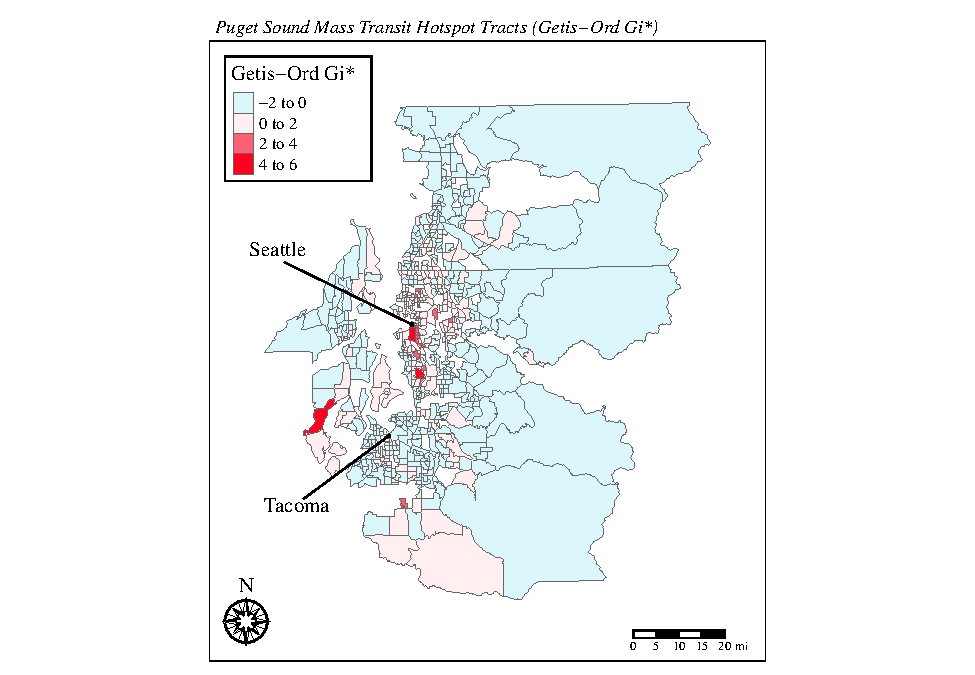
\includegraphics{truncated_transit_hotspots_paper_files/figure-latex/unnamed-chunk-7-1.pdf}

As can be seen in the map above, I chose to give the tracts with
non-significant Gi* values directional coloration. Tracts with
non-significant negative values are light blue and tracts with
non-significant positive values are light pink.

Speaking of significant values, however, it is clear to see that the
predominant occurrences of clustering are nearby Seattle, with most
happening in South Seattle (noted earlier for having high population
density and relatively lower median incomes). There are a couple of
other instances of significant clustering towards the southwest corner
of the map, but I do not have an intuitive explanation for why those are
occurring there. More research on locations of transit lines and tract
characteristics would have to be done in order to get a better
understanding of what is happening.

In the next section, I will take my analysis further with a spatial
model that regresses mass transit percentage onto the independent
variables: population density, median income, and median age.

\subsection{Regression using Spatial Error Model and Spatial Lag
Model}\label{regression-using-spatial-error-model-and-spatial-lag-model}

\subsubsection{Spatial Lag Model}\label{spatial-lag-model}

A spatial lag model essentially includes the value of mass transit
percentage in surrounding tracts as defined by the spatial weights
matrix. This allows the model to take into account the spatial
clustering we saw in the Moran's I test and produce coefficients for the
other predictor variables that are more efficient and accurate. For this
testing, I will use the \texttt{lagsarlm()} function from the
\texttt{spatialreg} package. I will log both population density and
median income, which is a common practice for variables that are always
above 0 and can theoretically increase without limit.

\begin{verbatim}
## 
## Call:
## lagsarlm(formula = masstransit_perc ~ log(pop_per_sqmile) + log(medincomeE) + 
##     medageE, data = psrc_table_clean, listw = weights_clean)
## 
## Residuals:
##     Min      1Q  Median      3Q     Max 
## -8.7888 -4.1372 -2.0656  2.3349 61.9643 
## 
## Type: lag 
## Coefficients: (asymptotic standard errors) 
##                      Estimate Std. Error z value Pr(>|z|)
## (Intercept)          0.906643   8.856855  0.1024  0.91847
## log(pop_per_sqmile)  0.491216   0.229086  2.1442  0.03201
## log(medincomeE)     -0.250715   0.777386 -0.3225  0.74707
## medageE              0.038179   0.053273  0.7167  0.47358
## 
## Rho: 0.32971, LR test value: 37.7, p-value: 8.2494e-10
## Asymptotic standard error: 0.049143
##     z-value: 6.7092, p-value: 1.9574e-11
## Wald statistic: 45.013, p-value: 1.9574e-11
## 
## Log likelihood: -2055.995 for lag model
## ML residual variance (sigma squared): 42.829, (sigma: 6.5444)
## Number of observations: 621 
## Number of parameters estimated: 6 
## AIC: 4124, (AIC for lm: 4159.7)
## LM test for residual autocorrelation
## test value: 2.519, p-value: 0.11248
\end{verbatim}

As can be seen in this output, there are two predictors for which the
coefficient is statistically significant. These are the lag term (Rho),
as expected given the clustering already seen above, and the
log(pop\_per\_sqmile) term. The positive coefficient on
log(pop\_per\_sqmile) indicates that greater population density is
associated with greater mass transit percentage. This was hypothesized.
I will not directly try to interpret the values of the coefficients
because the spatial lag term makes direct interpretations inaccurate.
The other predictors are non-significant.

I will also calculate a pseudo \(R^2\) value for this regression model
using the formula \(1 - \frac{SSE}{TSS}\).

\begin{verbatim}
## Pseudo R-squared: 0.1069
\end{verbatim}

This indicates our model explains approximately 10\% of the variation
seen in the dependent variable, mass transit percentage.

From the relatively low r-squared values and the lack of statistical
significance in most of my predictors, it is clear to me that this
analysis would benefit from a new selection of predictor variables. A
simple first step in this direction would be to do a more thorough
analysis with the ACS demographic variables, but there are richer
extensions beyond this. There are a plethora of built-environment and
transportation-relevant variables that could be summarized per tract,
such as land use percentage (industrial, residential, commercial, etc.),
parking availability/price, and traffic congestion (particularly
relevant in Seattle, where buses and at-grade light rail are common),
among others. I believe the more model complexity is the answer here,
rather than simplicity. This is particularly true as the goal of the
analysis is to better understand what impacts transit usage, rather than
whether a single variable does or does not impact transit usage.

\section{Discussion and
Interpretation}\label{discussion-and-interpretation}

\subsection{Key Findings}\label{key-findings}

This investigation put into statistical terms a pattern that was (a)
probably easy to intuit and (b) visually apparent from the initial
mapping: high values of transit usage clusters close to city centers
(particularly for Seattle) in the Puget Sound region. A further
corroborating relationship was revealed with the SLM: that population
density is positively associated with mass transit usage.

The other predictor variables (median income and median age) were not
statistically significantly related to my outcome variable. The analysis
did not present me with any surprising or counterintuitive results,
merely a lack of significance for some of my variables.

\subsection{Implications/Areas for Future
Inquiry}\label{implicationsareas-for-future-inquiry}

With statistical evidence in favor of urban clustering of transit usage,
I can now confidently ask the question: ``what is it about urban areas
that encourages transit ridership?'' I believe this can be decomposed
into two pieces. First, there are likely certain pro-transit
characteristics of urban areas. A high density of stops and transfer
options mean transit is more convenient for riders, as does better
walkability and a lower distance between likely origin and destination.
On the other hand, some characteristics of urban areas have a more
anti-car flavor. Limited and expensive parking options are a good
example. If increasing transit adoption and usage is a priority (and it
should be, for sustainability and equitability reasons), further
research should investigate these characteristics to better understand
how to design desirable transit in areas with low usage rates.

This sort of investigation could remain a spatial one. I imagine a
survey of people in the region, each linked to a census tract, and would
imagine that their public transit usage considerations might vary with
geography. People in urban areas might consider transfer reliability,
walkability, or anti-car factors more than suburban or rural
respondents, who might be more interested in things like overall speed.
Seattle, in particular, has a big suburban population that commutes
either to the city or nearby tech campuses and, as we can see from the
initial choropleth mapping, tends to do so by car. A better
understanding of their reasons for this would allow for better policy
and infrastructure design to increase transit usage and adoption.

\section{Conclusion}\label{conclusion}

This report can be thought of as a jumping-off point for my personal
research interests. Having this sort of statistical and spatial
understanding of how transit usage is distributed in the region gives me
a concrete foundation off of which to build further analyses. Although I
did not find much in the way of interesting regression results, the
analysis has given me pause to consider what other types of variables
(especially outside of basic ACS demographics) might be useful and/or
interesting to consider adding to future work. Finally, I think the
number of questions that this analysis provokes within me will be
helpful for thinking about future research directions and how the relate
to policy decisions.

\section{References}\label{references}

\subsection{Data Sources}\label{data-sources-1}

\begin{enumerate}
\def\labelenumi{\arabic{enumi}.}
\tightlist
\item
  National Atlas of the United States. (2013). Cities and Towns of the
  United States, 2014. National Atlas of the United States. Available
  at: \url{http://purl.stanford.edu/bx729wr3020}.
\item
  Puget Sound Regional Council. (2023). Household travel survey program.
  Puget Sound Regional Council.
  \url{https://www.psrc.org/our-work/household-travel-survey-program}
\item
  U.S. Census Bureau. (n.d.). \emph{American Community Survey 5-year
  estimates: 2022}. U.S. Department of Commerce. Retrieved December 11,
  2024, from \url{https://data.census.gov/}
\end{enumerate}

\subsection{Programming
Languages/Software}\label{programming-languagessoftware}

\begin{enumerate}
\def\labelenumi{\arabic{enumi}.}
\tightlist
\item
  R Core Team (2024). \emph{R: A Language and Environment for
  Statistical Computing}. R Foundation for Statistical Computing,
  Vienna, Austria. \url{https://www.R-project.org/}.
\item
  RStudio Team. (2020). RStudio: Integrated Development for R. RStudio,
  PBC, Boston, MA. \url{http://www.rstudio.com/}.
\end{enumerate}

\subsection{R Packages}\label{r-packages}

\begin{enumerate}
\def\labelenumi{\arabic{enumi}.}
\tightlist
\item
  Baddeley A, Rubak E, Turner R (2015). \emph{Spatial Point Patterns:
  Methodology and Applications with R}. Chapman and Hall/CRC Press,
  London. ISBN 9781482210200,
  \url{https://www.routledge.com/Spatial-Point-Patterns-Methodology-and-Applications-with-R/Baddeley-Rubak-Turner/p/book/9781482210200/}.
\item
  Bivand R (2022). ``R Packages for Analyzing Spatial Data: A
  Comparative Case Study with Areal Data.'' \emph{Geographical
  Analysis}, \emph{54}(3), 488-518.
  \url{https://doi.org/10.1111/gean.12319}.
\item
  Bivand R, Millo G, Piras G (2021). ``A Review of Software for Spatial
  Econometrics in R.'' \emph{Mathematics}, \emph{9}(11).
  \url{https://doi.org/10.3390/math9111276},
  \url{https://www.mdpi.com/2227-7390/9/11/1276}.
\item
  Bivand R, Pebesma E, Gómez-Rubio V (2013). \emph{Applied spatial data
  analysis with R, Second edition}. Springer, NY.
  \url{https://asdar-book.org/}.
\item
  Bivand R, Wong D (2018). ``Comparing implementations of global and
  local indicators of spatial association.'' \emph{TEST}, \emph{27}(3),
  716-748. \url{https://doi.org/10.1007/s11749-018-0599-x}.
\item
  Müller K (2020). \emph{here: A Simpler Way to Find Your Files}. R
  package version 1.0.1, \url{https://CRAN.R-project.org/package=here}.
\item
  Pebesma, E., \& Bivand, R. (2023). Spatial Data Science: With
  Applications in R. Chapman and Hall/CRC.
  \url{https://doi.org/10.1201/9780429459016}
\item
  Pebesma E, Bivand R (2023). \emph{Spatial Data Science With
  Applications in R}. Chapman \& Hall.
  \url{https://r-spatial.org/book/}.
\item
  Pebesma, E., 2018. Simple Features for R: Standardized Support for
  Spatial Vector Data. The R Journal 10 (1), 439-446,
  \url{https://doi.org/10.32614/RJ-2018-009}
\item
  Tennekes M (2018). ``tmap: Thematic Maps in R.'' \emph{Journal of
  Statistical Software}, \emph{84}(6), 1-39.
  \url{https://doi.org/10.18637/jss.v084.i06}.
\item
  Walker K, Herman M (2024). \emph{tidycensus: Load US Census Boundary
  and Attribute Data as `tidyverse' and `sf'-Ready Data Frames}. R
  package version 1.6.7,
  \url{https://CRAN.R-project.org/package=tidycensus}.
\item
  Wickham H (2023). \emph{forcats: Tools for Working with Categorical
  Variables (Factors)}. R package version 1.0.0,
  \url{https://CRAN.R-project.org/package=forcats}.
\item
  Wickham H, Averick M, Bryan J, Chang W, McGowan LD, François R,
  Grolemund G, Hayes A, Henry L, Hester J, Kuhn M, Pedersen TL, Miller
  E, Bache SM, Müller K, Ooms J, Robinson D, Seidel DP, Spinu V,
  Takahashi K, Vaughan D, Wilke C, Woo K, Yutani H (2019). ``Welcome to
  the tidyverse.'' \emph{Journal of Open Source Software}, \emph{4}(43),
  1686. \url{https://doi.org/10.21105/joss.01686}.
\item
  Xie Y (2024). \emph{knitr: A General-Purpose Package for Dynamic
  Report Generation in R}. R package version 1.48,
  \url{https://yihui.org/knitr/}.
\item
  Yihui Xie (2015) Dynamic Documents with R and knitr. 2nd edition.
  Chapman and Hall/CRC. ISBN 978-1498716963
\item
  Yihui Xie (2014) knitr: A Comprehensive Tool for Reproducible Research
  in R. In Victoria Stodden, Friedrich Leisch and Roger D. Peng,
  editors, Implementing Reproducible Computational Research. Chapman and
  Hall/CRC. ISBN 978-1466561595
\end{enumerate}

\end{document}
